\documentclass[a4paper, 14pt,russian]{extarticle}

\usepackage[russian]{babel}
\usepackage[T2A]{fontenc}
\usepackage[utf8]{inputenc}
%Соответствующий математический шрифт для Times new roman
\usepackage{newtxmath}
\usepackage{fontspec} 
\usepackage{multirow}
%\usepackage{polyglossia}
%Times new roman
\defaultfontfeatures{Ligatures={TeX},Renderer=Basic} 
\setmainfont[Ligatures={TeX,Historic}]{Times New Roman}
\setmainfont{Times New Roman}
\setsansfont{Arial}
\setmonofont{Courier New}
\newfontfamily\cyrillicfont[Script=Cyrillic]{Times New Roman}
\newfontfamily\cyrillicfontsf[Script=Cyrillic]{Arial}
\newfontfamily\cyrillicfonttt[Script=Cyrillic]{Courier New}

%\setdefaultlanguage{russian}

%Геометрия
\usepackage{geometry}
\geometry{top=20mm}
\geometry{bottom=15mm}
\geometry{left=20mm}
\geometry{right=15mm}
\usepackage{setspace}
%Нормальные дроби через запятую
\usepackage{ncccomma}

\newcommand{\changefont}{%
	\fontsize{12}{11}\selectfont
}

%Заголовки
\usepackage{fancyhdr}
\pagestyle{fancy}
\fancyhf{}
%\renewcommand{\sectionmark}[1]{\markright{#1}}
\fancyhead[R]{\changefont \slshape \leftmark}
\fancyhead[L]{\changefont \slshape \rightmark}
%\newcommand{\ssubsection}[1]{\subsection*{#1}
%	\addcontentsline{toc}{subsection}{#1}
%	\markright{#1}{}}
\cfoot{\thepage}

%\полуторный интервал
\setstretch{1.15}
\setlength{\parindent}{1.25cm}

\usepackage{amsmath, amsfonts, mathtools}
\usepackage{physics}
\usepackage{indentfirst}
\usepackage{xcolor}
\usepackage{alltt}
\usepackage{graphicx}
\usepackage{wrapfig}
\usepackage{pgfplots}

%Настройка ссылок
\usepackage{hyperref}
%\usepackage{upgreek}
%\renewcommand{\beta}{\upbeta}
\hypersetup{
	colorlinks,
	citecolor=black,
	filecolor=black,
	linkcolor=black,
	urlcolor=black
}
\usepackage{caption}
\DeclareCaptionLabelSeparator{dot}{. }
\captionsetup{justification=centering,labelsep=dot}
\usepackage{titlesec}

%Формат заголовков
\titleformat{\section}{\bfseries\filcenter\Large}{\thesection}{1em}{}
\titleformat{\subsection}{\bfseries\filcenter\large}{\thesubsection}{1em}{}
\titleformat{\subsubsection}{\bfseries\filcenter\normalsize}{\thesubsubsection}{1em}{}

\usepackage{chngcntr}

%Включить в нумерацию картинок раздел
\counterwithin{figure}{section}

%Листинги кода и их стили
\usepackage{listings}
\usepackage{minted}
\lstdefinestyle{c++} {
	language=C++,
	breaklines=true,
	frame=single,
	numbers=left,
	basicstyle=\footnotesize\ttfamily,
	keywordstyle=\bfseries\color{green!40!black},
	commentstyle=\itshape\color{purple!40!black},
	identifierstyle=\color{blue},
	backgroundcolor=\color{gray!10!white},
}

\lstdefinestyle{python}{
	language=Python,
	breaklines=true,
	frame=single,
	numbers=left,
	keywordstyle=\bfseries\color{green!40!black},
	frame=lines,
	basicstyle=\footnotesize\rmfamily
}

\lstdefinestyle{cmd}{
	breaklines=true,
	frame=single,
	basicstyle=\footnotesize\ttfamily,
	frame=lines
	basicstyle=\footnotesize
}

\begin{document}
	
	\begin{titlepage}
	\newpage
	\begin{center}
		
\includegraphics[width=\textwidth]{png/tit.png}
		Институт информационных и вычислительных технологий \\
		Кафедра управления и интеллектуальных технологий
		\vspace{1.25cm}
	\end{center}
	
	\vspace{1.2em}
	
	\begin{center}
		%\textsc{\textbf{}}
		\begin{spacing}{1}
			{\Large Лабораторная работа №2\linebreak
				По дисциплине <<Теория автоматического управления>> \\}
			\large{\bf<<Анализ динамики нелинейных систем методом фазовой плоскости>>}
		\end{spacing}
	\end{center}
	
	\vspace{5em}
	
	
	\vspace{6em}
	
	\noindent Выполнили студенты: Михайловский М., Томчук В. \\
	Группа: А-03-21 \\
	Бригада: 1\\
	Проверил: Деменьтьев В.\,Ю.
	
	
	\vspace{\fill}
	
	\begin{center}
		Москва 2024
	\end{center}
	
\end{titlepage}
	\setcounter{page}{2}
	\pagenumbering{arabic}
	\tableofcontents
	\newpage
	
	\section{Постановка задачи}
	
	Задана линейная система, описываемая следующим уравнением:
	\begin{equation*}
		y''+a_1y'+a_0y = 0
	\end{equation*}
	
	Подобрать коэффициенты $a_0,\,a_1$, для двух видов особой точки: \textbf{центр и неустойчивый узел}. Исследовать фазовые портреты и переходные процессы полученных линейных систем методом фазовой плоскости. 
	
	\section{Выполнение работы}
	\subsection{Подготовка к работе}
	
	\underline{Центр}. Для рассматриваемой системы характеристическое уравнение (ХУ) имеет следующий вид:
	\begin{equation*}
		p^2 + a_1p + a_0 = 0 \Leftrightarrow (p-p_1)(p-p_2) = 0
	\end{equation*}

	Особой точкой линейной системы будет центр, если корни ХУ будут мнимыми. Выберем $p_{1,2} = \pm j\sqrt{6}$. Тогда, раскрывая скобки, получим коэффициенты $a_0,\,a_1$:
	\begin{equation*}
		(p-j\sqrt{6})(p+j\sqrt{6}) = p^2 + 6 = 0 \Rightarrow a_1 = 0,\, a_0 = 6 \Rightarrow
	\end{equation*}
	\begin{equation*}
		\Rightarrow y'' + 6y = 0
	\end{equation*}

	Тогда соответствующая система в нормальной форме Коши ($y=y_1$):
	\begin{equation}
		\begin{cases*}
			\dfrac{dy_1}{dt} = y_2 \\[0.5em] 
			\dfrac{dy_2}{dt} = -6y_1
		\end{cases*}
		\label{center}
	\end{equation}

	\underline{Неустойчивый узел}. Особой точкой линейной системы будет неустойчивый узел, если корни ХУ будут действительными положительными. Пусть $p_{1,2} = 1,\,2$. Получим по теореме Виета следующее характеристическое уравнение:
	\begin{equation*}
		p^2-3p+2 = 0 \stackrel{\mathcal{L}^{-1}}{\to} y''-3y'+2y = 0 \Rightarrow a_1=-3,\,a_0=2
	\end{equation*}

	В нормальной форме Коши система имеет вид ($y=y_1$):
	\begin{equation}
		\begin{cases*}
			\dfrac{dy_1}{dt} = y_2 \\[0.5em] 
			\dfrac{dy_2}{dt} = -2y_1+3y_2
		\end{cases*}
		\label{uzel}
	\end{equation}

	\subsection{Анализ результатов работы}
	\subsubsection{Особая точка центр}
	
	Исследования проводились при помощи компьютерного моделирования. Введённые параметры, в соответствии с полученной системой (\ref{center}) представлены на рис. \ref{params1}.
	
	\begin{figure}[h]
		\centering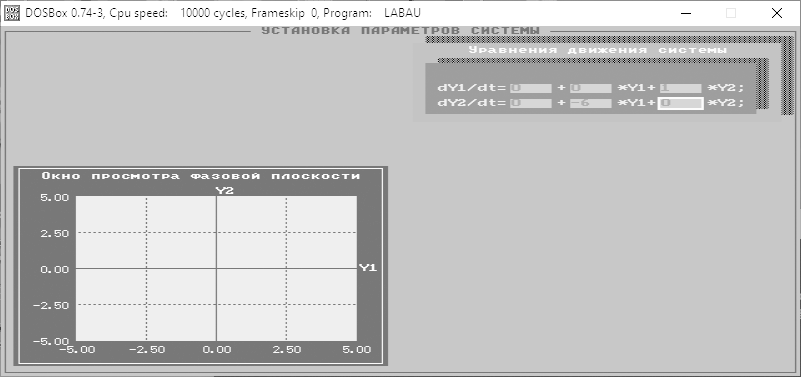
\includegraphics[width=.7\textwidth,trim={300px 190px 20px 33px},clip]{Центр/Параметры.png}
		\caption{Установленные параметры исследуемой системы}
		\label{params1}
	\end{figure}

	Затем для различных начальных условий численным моделированием было получено семейство фазовых траекторий заданной системы рис. \ref{portret1}.
	
	\begin{figure}[h]
		\centering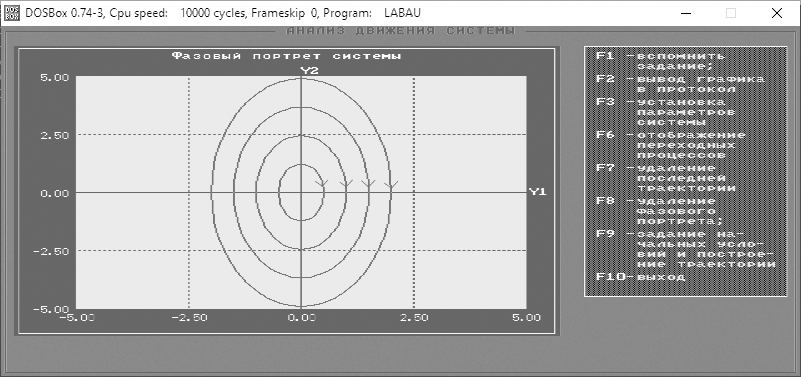
\includegraphics[width=.6\textwidth,trim={0 0 165px 20px},clip]{Центр/Портрет.png}
		\caption{Полученный фазовый портрет системы}
		\label{portret1}
	\end{figure}

	Семейство интегральных кривых имеет вид эллипсов, в данном случае, вытянутых вдоль оси $y_2$. Соотношение длин полуосей эллипсов фазовых траекторий для данной особой точки зависит от конкретных параметров системы и может быть любым.
	
	Далее были построены переходные характеристики (рис. \ref{pereh1})
	\vspace{0.5em}
	
	\noindent\begin{minipage}[h]{.5\textwidth}
		\centering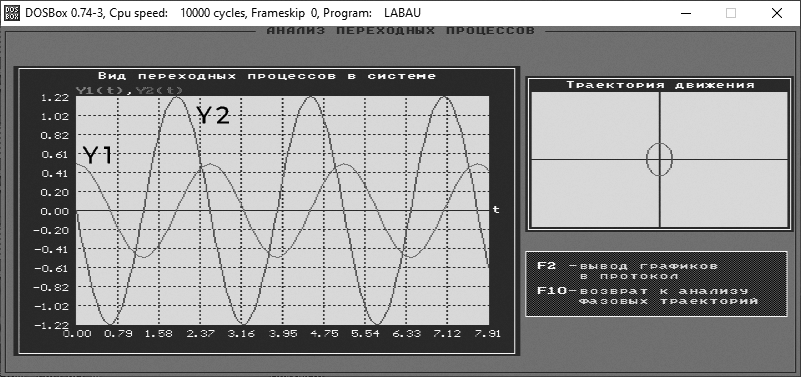
\includegraphics[width=.98\textwidth,trim={0 0 0 20px},clip]{Центр/переходной1.png}
		\centering{а)}
	\end{minipage}
	\begin{minipage}[h]{.5\textwidth}
		\centering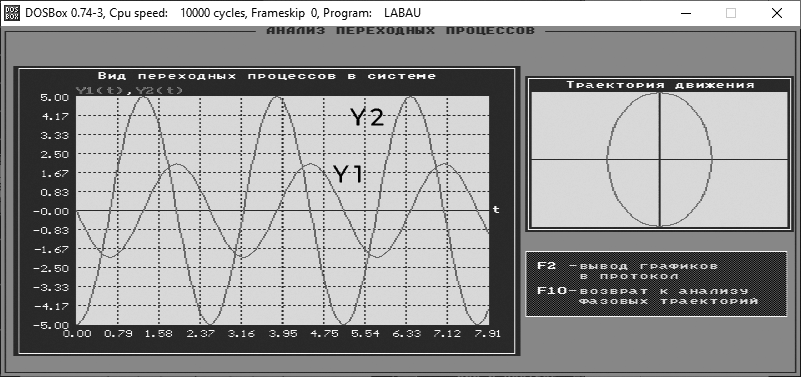
\includegraphics[width=.98\textwidth,trim={0 0 0 20px},clip]{Центр/переходной2.png}
		\centering{б)}
	\end{minipage}
	{\captionof{figure}{Переходные характеристики для системы с особой точкой центр}
	\label{pereh1}}

	\vspace{0.5em}
	Видно, что система является устойчивой по Ляпунову, но не является асимптотически устойчивой. Это следует из того, что переменные состояния изменяются по гармоническому закону и являются незатухающими.
	
	\subsubsection{Особая точка неустойчивый узел}
	
	Введённые параметры, в соответствии с полученной системой (\ref{uzel}) представлены на рис. \ref{params2}.
	
	\begin{figure}[h]
		\centering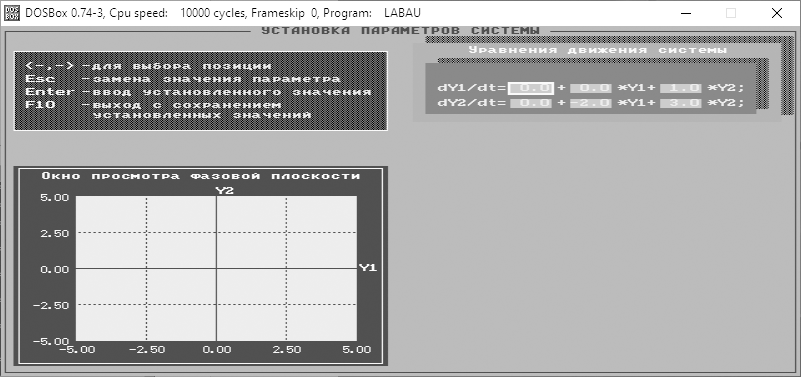
\includegraphics[width=.7\textwidth,trim={300px 190px 20px 33px},clip]{Узел/Параметры.png}
		\caption{Установленные параметры исследуемой системы}
		\label{params2}
	\end{figure}
	
	Затем для различных начальных условий численным моделированием было получено семейство фазовых траекторий заданной системы рис. \ref{portret2}.
	
	\begin{figure}[h]
		\centering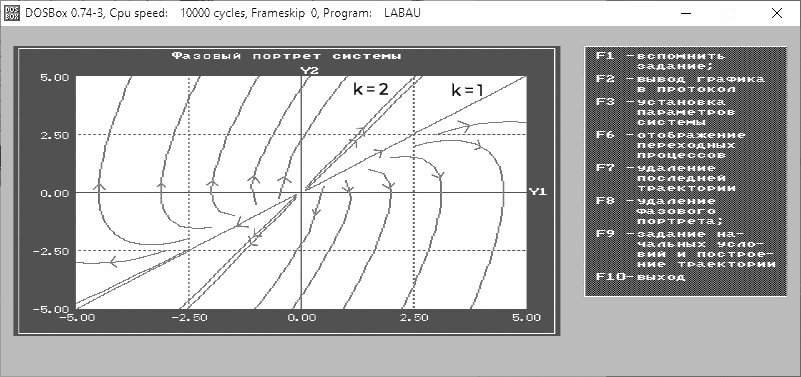
\includegraphics[width=.6\textwidth,trim={0 0 165px 20px},clip]{Узел/Портрет.png}
		\caption{Полученный фазовый портрет системы}
		\label{portret2}
	\end{figure}
	
	Данное семейство представляет собой кривые параболического типа. Асимптотами являются прямые с углами наклона равными собственным числам матрицы из матричного представления системы (\ref{uzel}) или, что то же, корням ХУ. 
	
	Для исследуемой системы матричное представление следующее:
	\begin{equation*}
		\vec{y}' = A\vec{y},\; \vec{y} = \begin{pmatrix}y_1 \\ y_2\end{pmatrix},\; A=\begin{pmatrix}0 & 1 \\ -2 & 3\end{pmatrix}\,.
	\end{equation*}
	
	Далее были построены переходные характеристики (рис. \ref{pereh2})
	\vspace{0.5em}
	
	\noindent\begin{minipage}[h]{.5\textwidth}
		\centering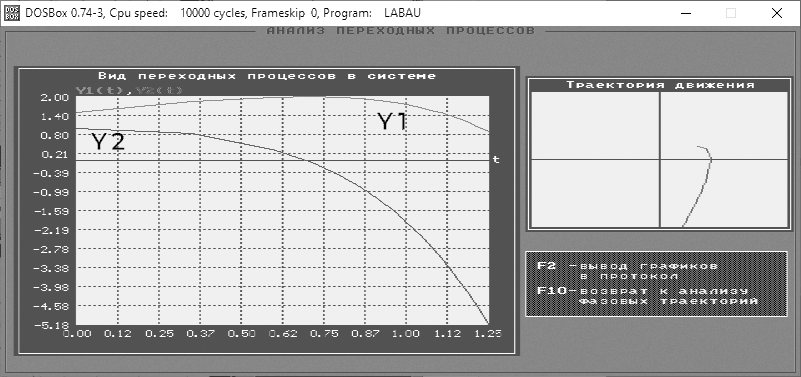
\includegraphics[width=.98\textwidth,trim={0 0 0 20px},clip]{Узел/переходной1.png}
		\centering{а)}
	\end{minipage}
	\begin{minipage}[h]{.5\textwidth}
		\centering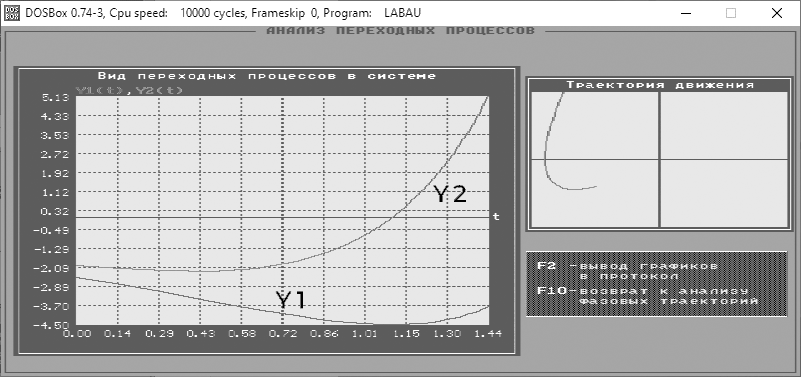
\includegraphics[width=.98\textwidth,trim={0 0 0 20px},clip]{Узел/переходной2.png}
		\centering{б)}
	\end{minipage}
	{\captionof{figure}{Переходные характеристики для системы с особой точкой центр}
		\label{pereh2}}
	
	\vspace{0.5em}
	Видно, что система является неустойчивой и, вообще говоря, имеет неустойчивую особую точку $\vec{y}^\intercal = \begin{pmatrix}0 & 0\end{pmatrix}$
	
	\subsubsection{Выводы}
	
	Было исследовано применение метода фазовой плоскости на примере линейных систем. Как и ожидалось, для системы с характеристическими корнями на мнимой оси был получен вывод о граничной устойчивости, а для системы с правыми корнями вывод о неустойчивости.
	
	Также, данный метод помимо исследования устойчивости даёт возможность получить вид переходного процесса, что является важной характеристикой системы. 
	
\end{document}
